%%%%%%%%%%%%%%%%%%%%%%%%%%%%%%%%%%%%%%%%%%%%%%%%%%%%%%%%%%%%%%%%%%%%%%%%%
% Template for a classical article
%%%%%%%%%%%%%%%%%%%%%%%%%%%%%%%%%%%%%%%%%%%%%%%%%%%%%%%%%%%%%%%%%%%%%%%%%
\documentclass[12pt,a4paper,notitlepage,onecolumn]{article}
%%%%%%%%%%%%%%%%%%%%%%%%%%%%%%%%%%%%%%%%%%%%%%%%%%%%%%%%%%%%%%%%%%%%%%%%%
\newcommand{\Author}{Fabio Zanini}
\newcommand{\Title}{Multi-template Models}
%%%%%%%%%%%%%%%%%%%%%%%%%%%%%%%%%%%%%%%%%%%%%%%%%%%%%%%%%%%%%%%%%%%%%%%%%
\usepackage[english]{babel}
\usepackage[utf8x]{inputenc}
\usepackage{amsmath,amsfonts,amssymb,eucal,eurosym}
\usepackage{color}
\usepackage{graphicx}
\usepackage[font=small, format=hang, labelfont={sf,bf}, figurename=Fig.]{caption}
%\usepackage{cite}
%\usepackage{epigraph}
%\setlength{\epigraphwidth}{.55\textwidth}
%\setlength{\epigraphrule}{0pt}
%\usepackage{multirow}
%\usepackage[version=3]{mhchem}
%\usepackage{sagetex}
\usepackage[	colorlinks,linkcolor=red,citecolor=red]{hyperref}
\hypersetup{	pdfauthor={\Author}, pdftitle={\Title}, pdfkeywords={\Keywords}	}
%%%%%%%%%%%%%%%%%%%%%%%%%%%%%%%%%%%%%%%%%%%%%%%%%%%%%%%%%%%%%%%%%%%%%%%%%
\graphicspath{{./figures/}}
%%%%%%%%%%%%%%%%%%%%%%%%%%%%%%%%%%%%%%%%%%%%%%%%%%%%%%%%%%%%%%%%%%%%%%%%%
%\DeclareMathOperator\de{d\!}
%\newcommand{\comment}[1]{\textit{\textcolor{red}{#1}}}
%%%%%%%%%%%%%%%%%%%%%%%%%%%%%%%%%%%%%%%%%%%%%%%%%%%%%%%%%%%%%%%%%%%%%%%%%
\title{\Title}
\author{\Author}
\date{\today}
%%%%%%%%%%%%%%%%%%%%%%%%%%%%%%%%%%%%%%%%%%%%%%%%%%%%%%%%%%%%%%%%%%%%%%%%%
\begin{document}
\maketitle

\begin{figure}[h!]
 \begin{center}
  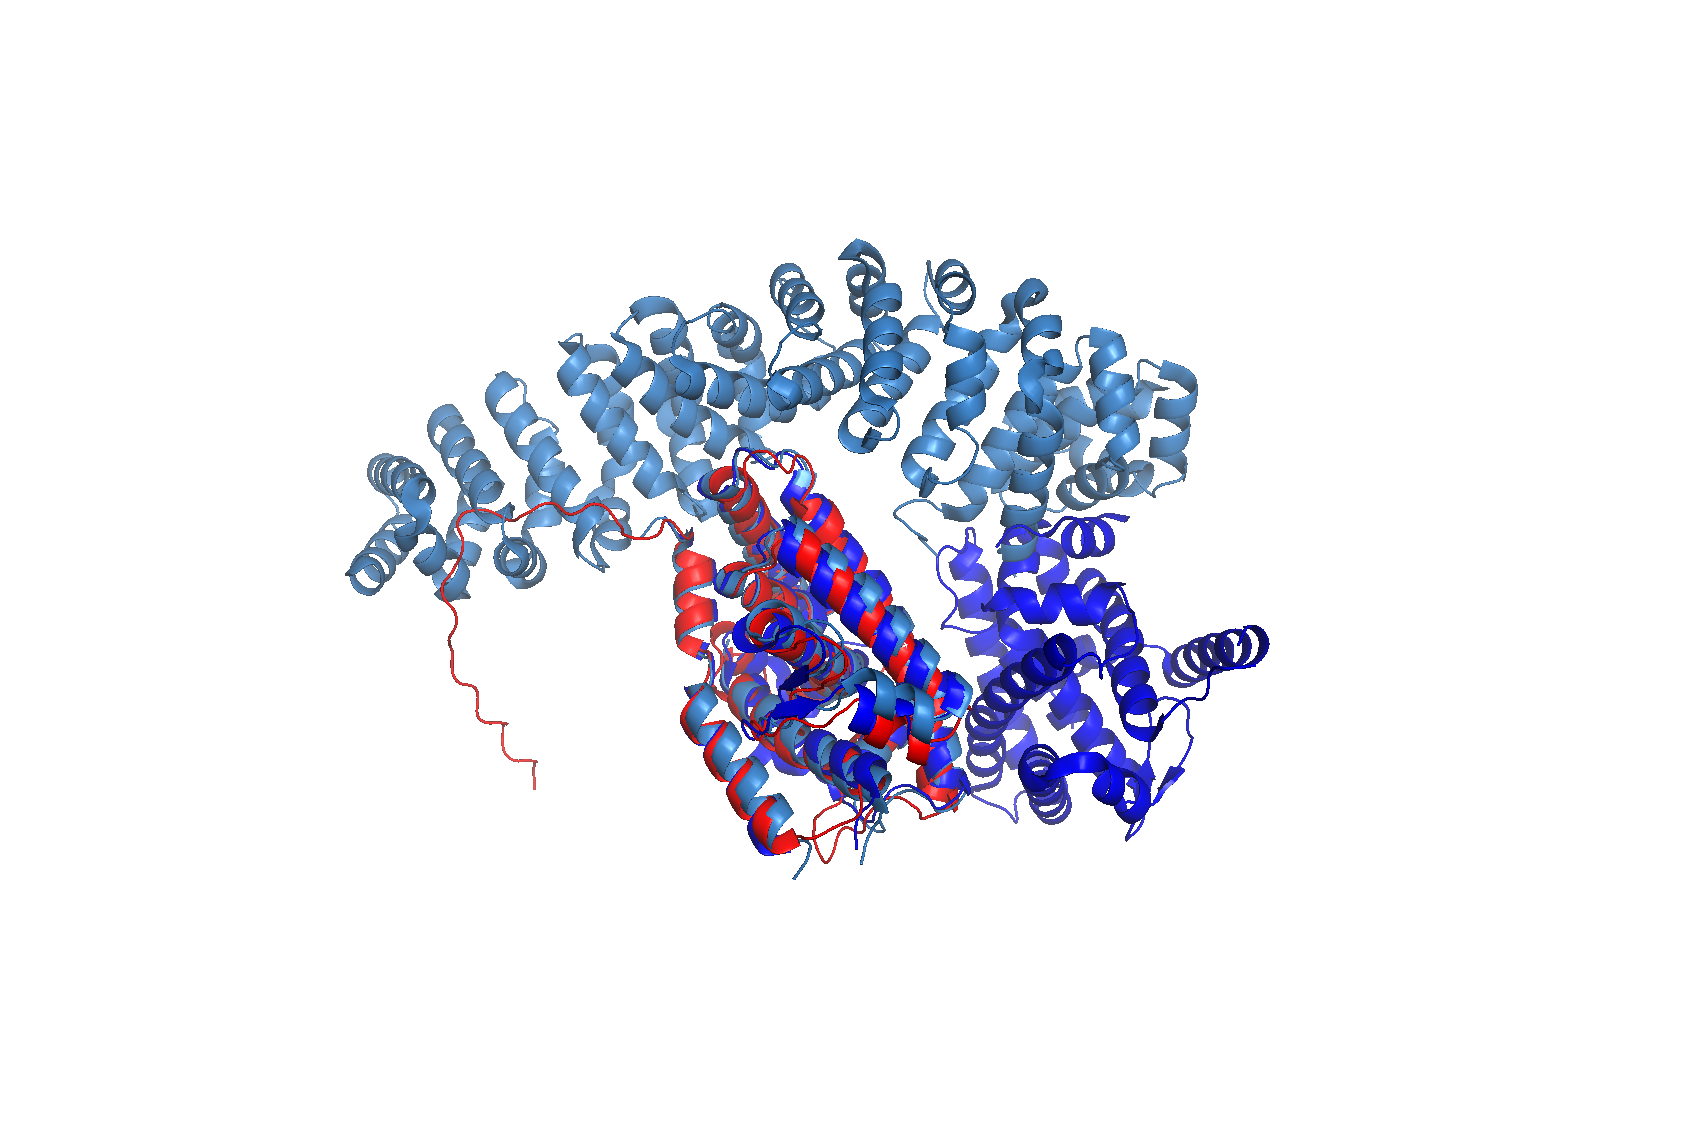
\includegraphics[width=0.8\linewidth]{1yje_A-multiple_n_2.png}
  \caption{Example of a multiple model, our unknown sequence threaded onto 3XT7 and 3PLZ. Colors: red = our model, blue = templates.}
  \label{fig:1yje_A-multiple_n_2}
 \end{center}
\end{figure}
I have written a script that uses more than one model into a sequence/structure MSA and then threads our unknown sequence onto the alignment of all structures (somehow). An example using only two templates is shown in \figurename~\ref{fig:1yje_A-multiple_n_2}.

\begin{figure}[h!]
 \begin{center}
  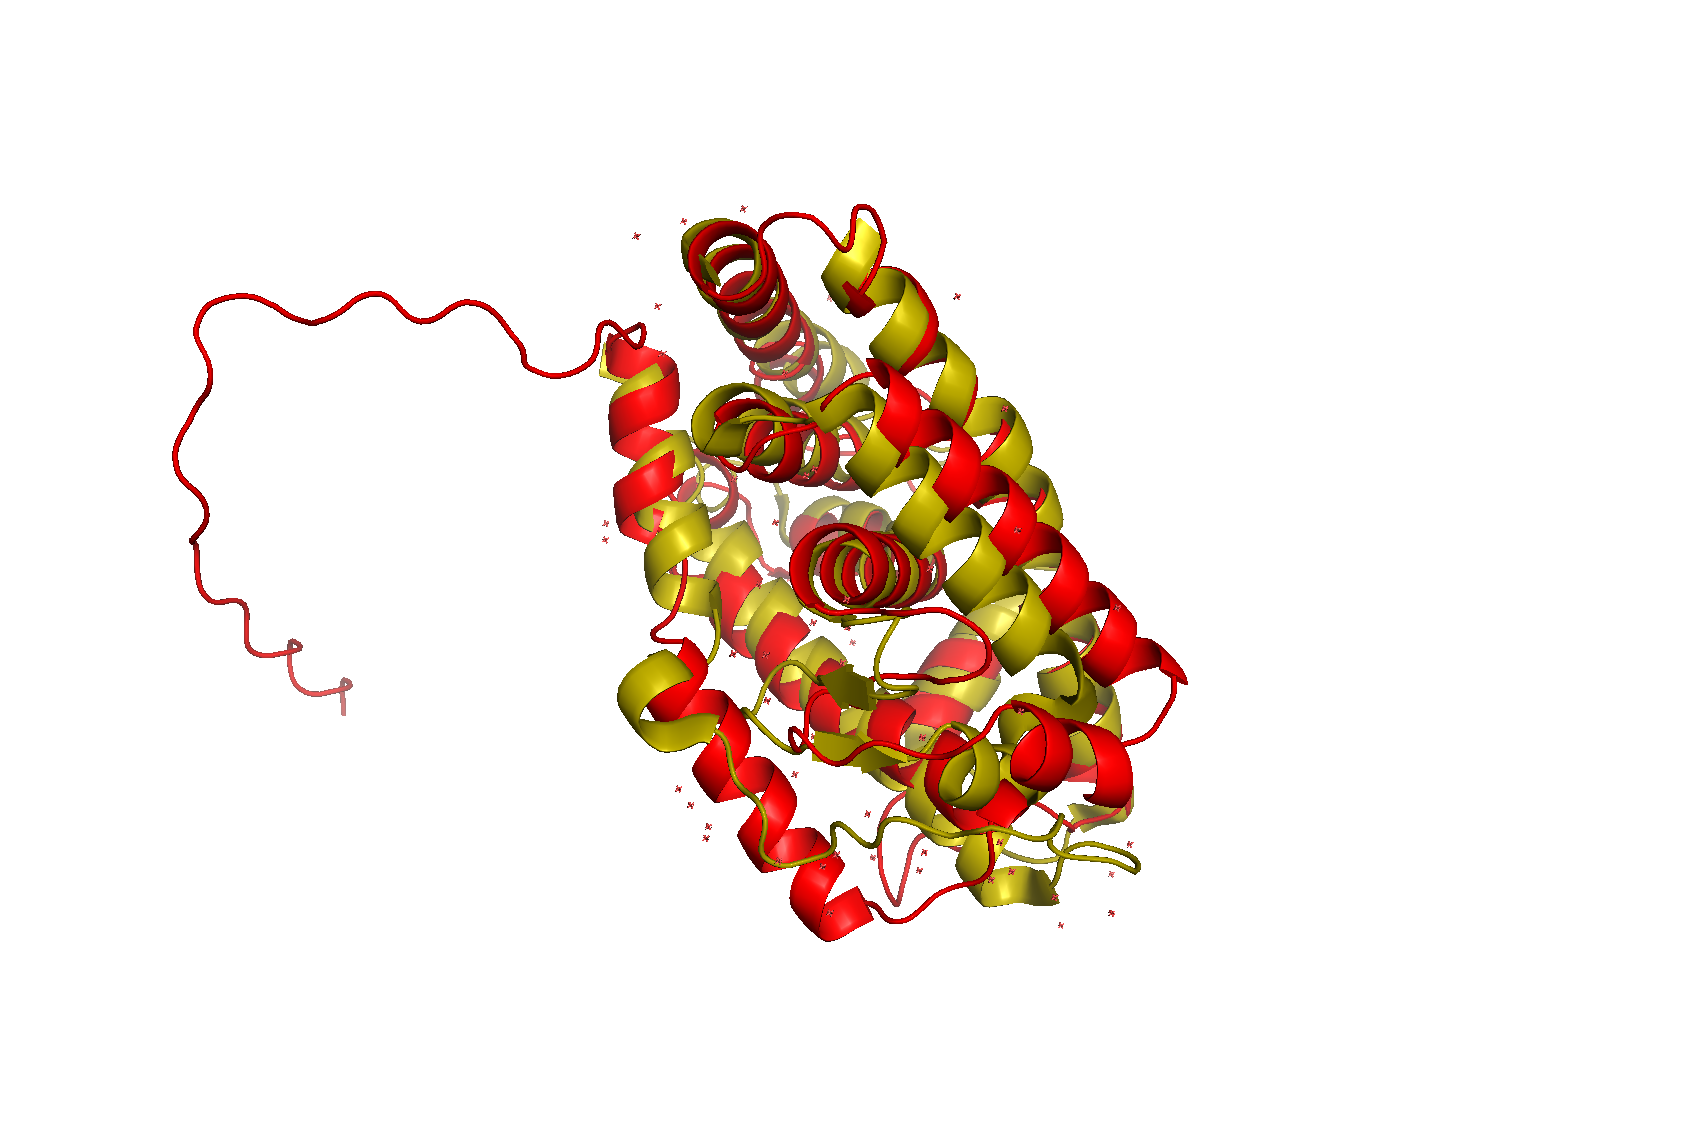
\includegraphics[width=0.45\linewidth]{prediction_truth.png}
  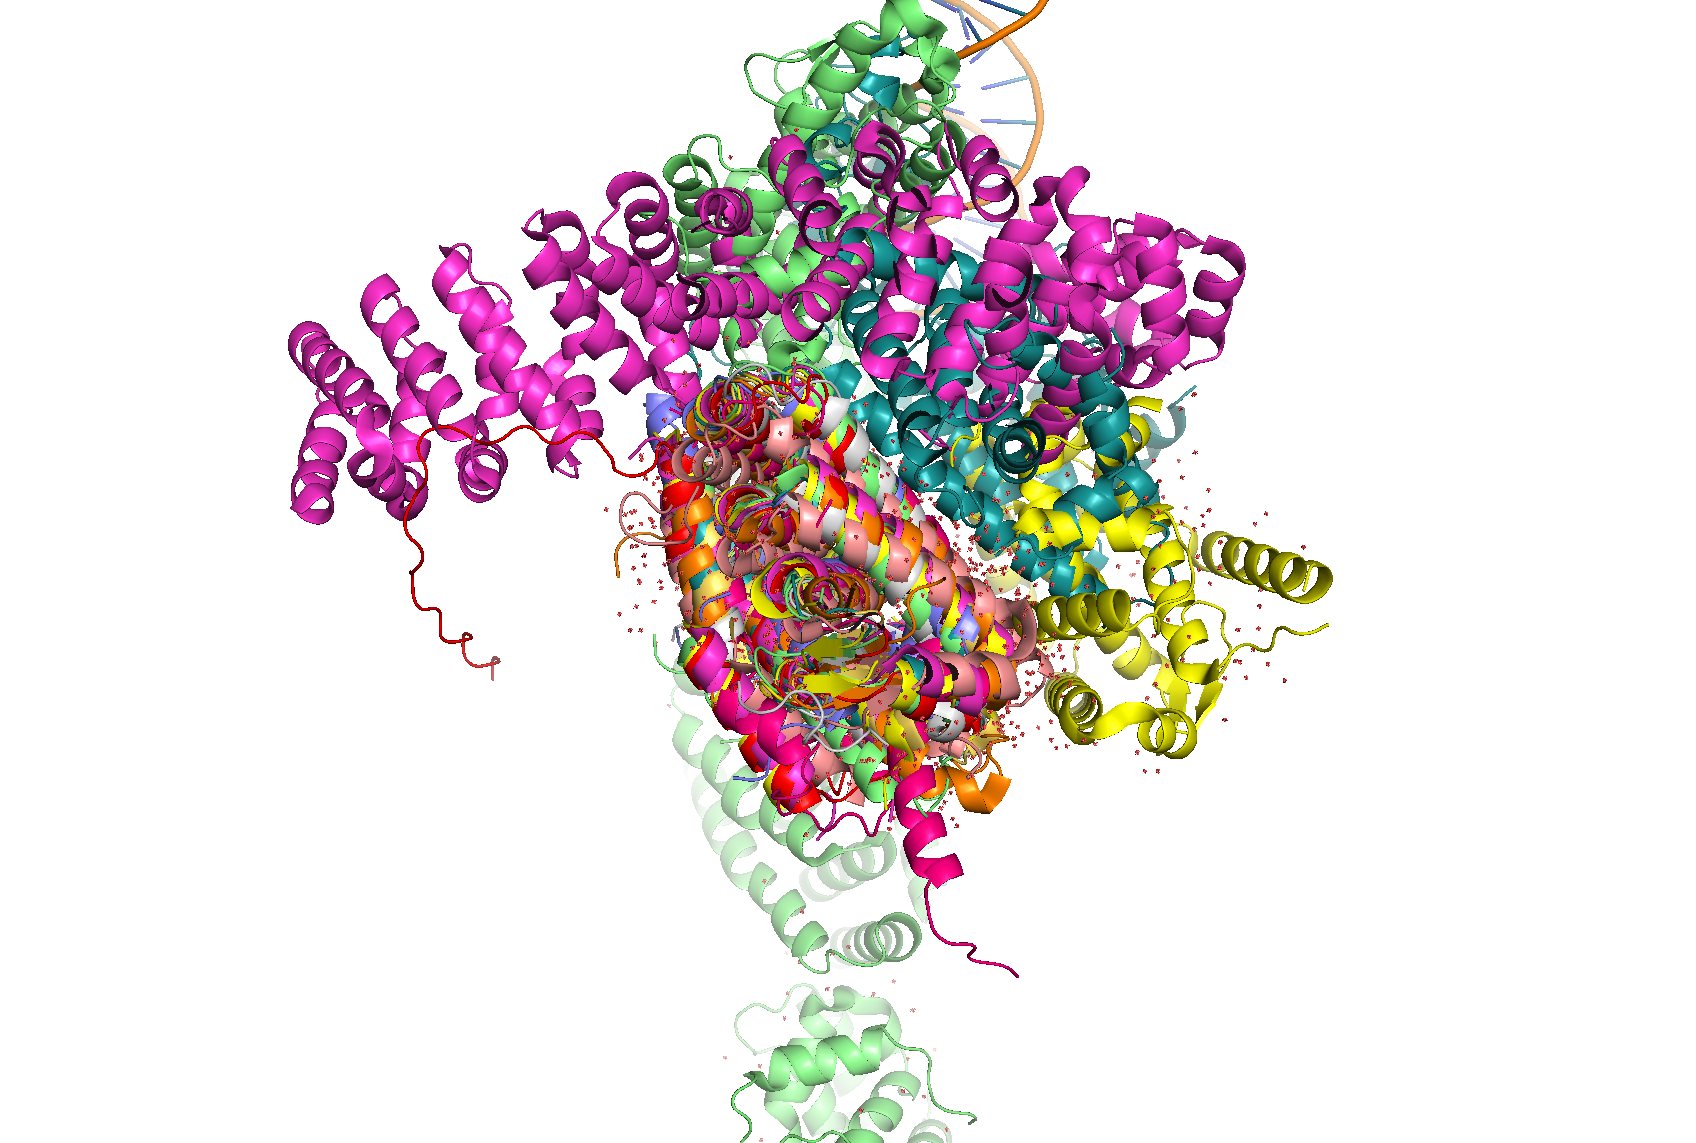
\includegraphics[width=0.45\linewidth]{prediction_templates.png}
  \caption{Example of a mult5iple model, our unknown sequence threaded onto ten similar PDB entries. Left hand side: the predicted structure against the true one; right hand side: the same against all ten models. Colors: red = our model, gold = true structure, other = templates.}
  \label{fig:tt}
 \end{center}
\end{figure}
 I have also written a small pymol script that outputs figures of a) the original structure with the predicted one and b) all templates with the predicted one. The results are presented in \figurename~\ref{fig:tt}.

We still need to ``present results in a convenient way''. According to Sven's hint, this should amount to calculate overlap between our predicted sites and the true structure, or the templates...? The latter seems to be a silly way of evaulating a prediction, but -- oh, well.

Modeller includes a few methods to assess the quality of the model. I am not convinced they are a good idea, but they seem to swin in the direction wished by our advisor. I finally generate multiple (3) multi-template models using 15 templates (including the true structure) and select the one with the top DOPE score (see in papers, Shen and Sali 2006). The result in \figurename~\ref{fig:tt_DOPE}.
\begin{figure}[h!]
 \begin{center}
  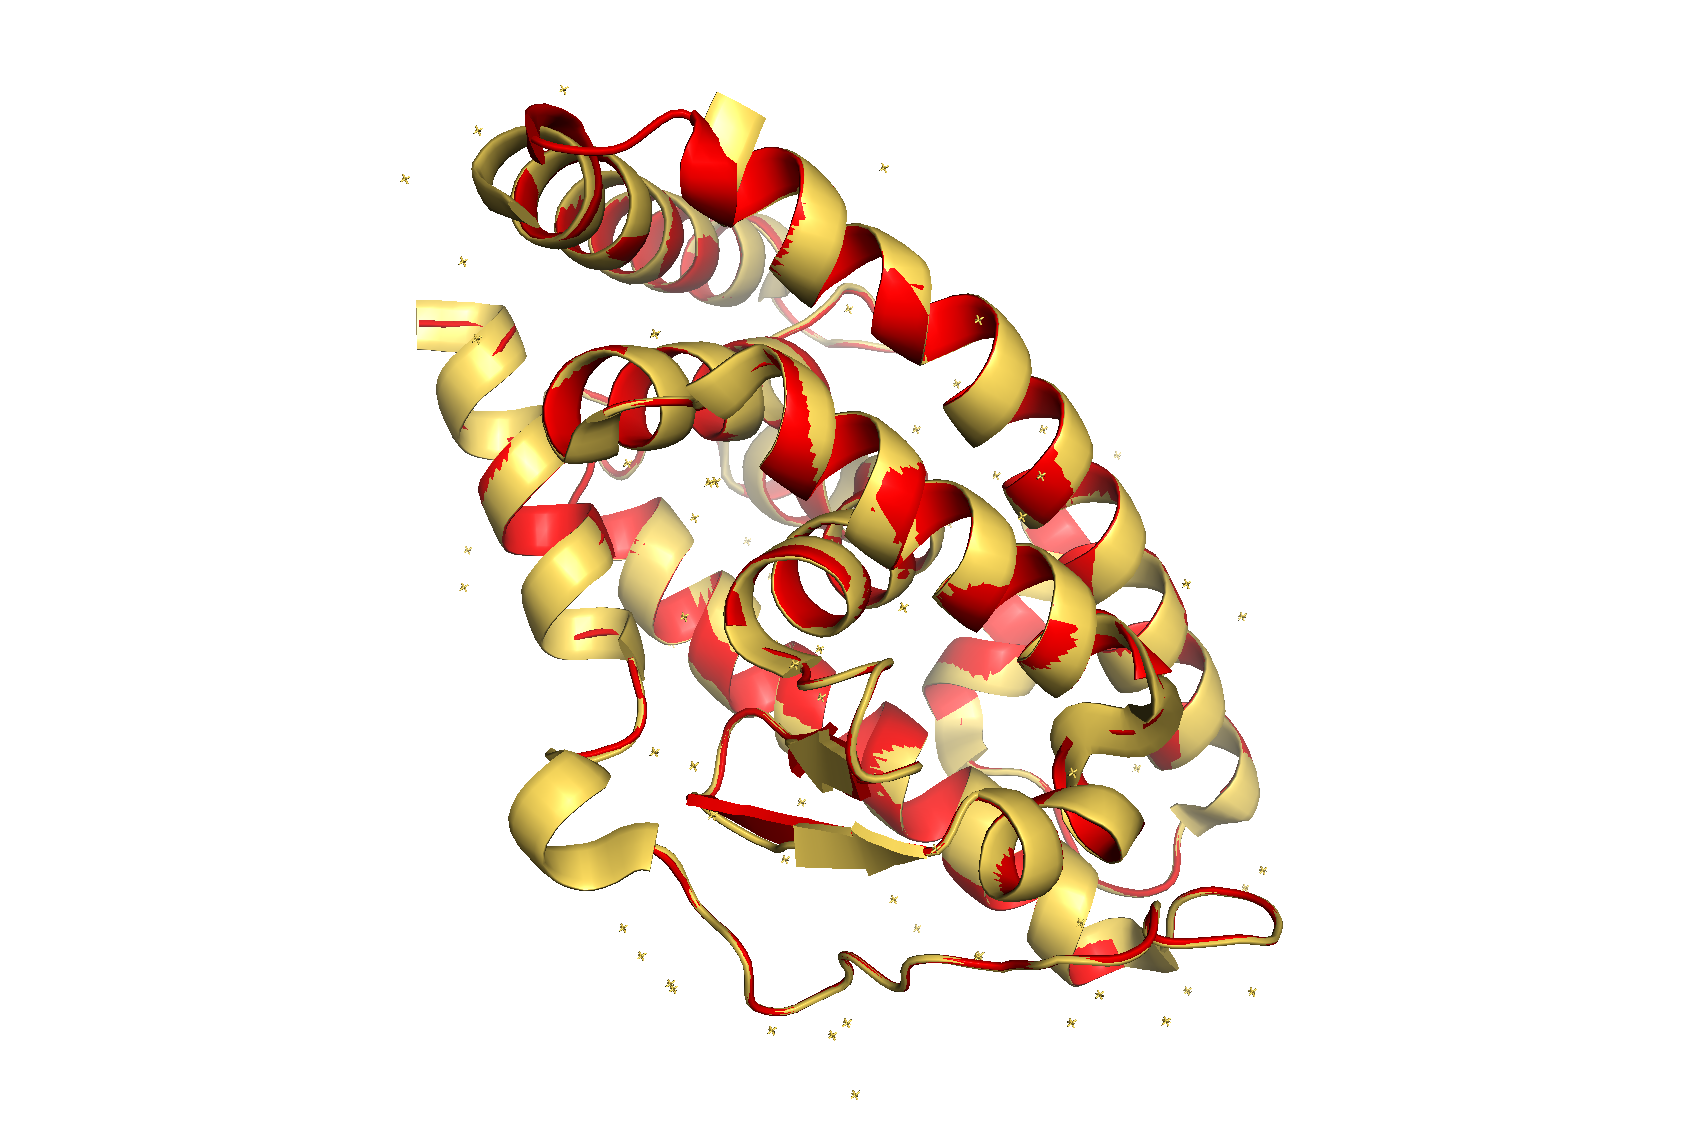
\includegraphics[width=0.45\linewidth]{prediction_truth_DOPE.png}
  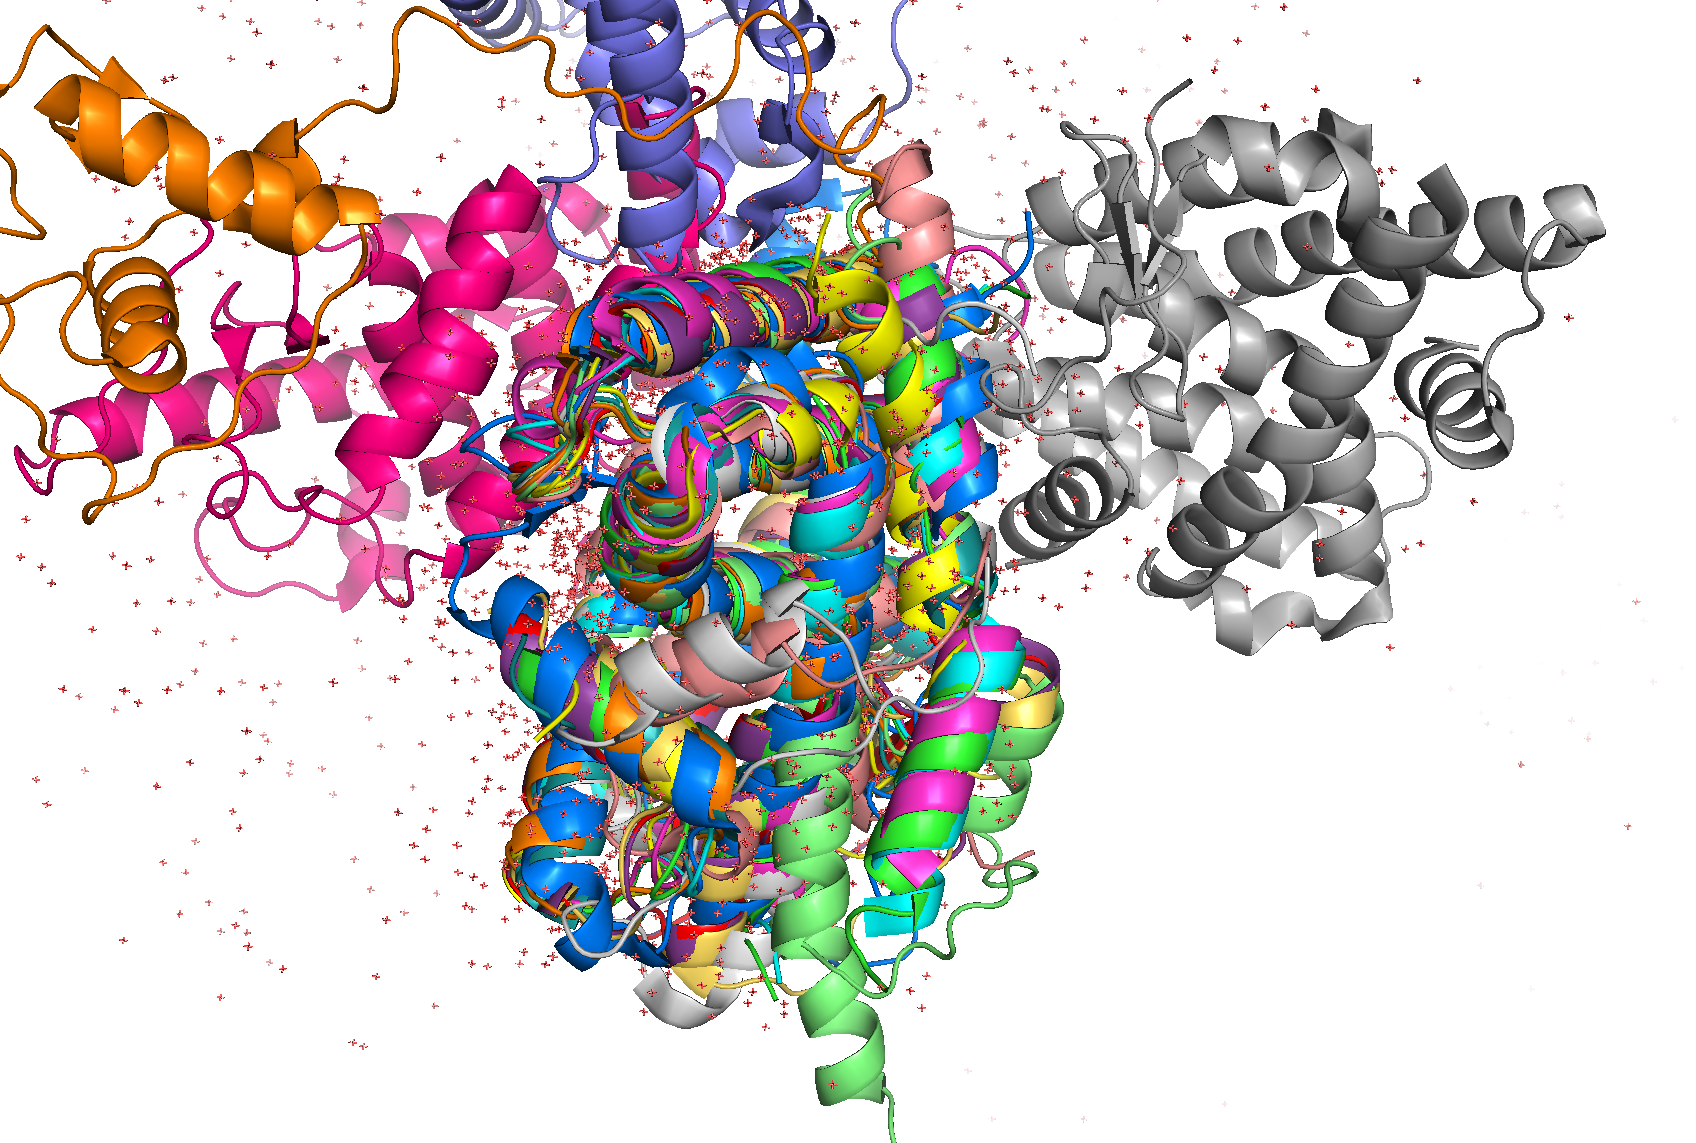
\includegraphics[width=0.45\linewidth]{prediction_templates_DOPE.png}
  \caption{Example of a mult5iple model, our unknown sequence threaded onto 15 similar PDB entries. Left hand side: the predicted structure against the true one; right hand side: the same against all 15 models. Colors: red = our model, gold = true structure, other = templates.}
  \label{fig:tt_DOPE}
 \end{center}
\end{figure}
Of course, the prediction matches the true structure perfectly, because we included it in the list of templates, and it is assigned an overwhelming high weight because of the high (full) sequence similarity.

\end{document}

